\documentclass{article}\usepackage[]{graphicx}\usepackage[]{color}
%% maxwidth is the original width if it is less than linewidth
%% otherwise use linewidth (to make sure the graphics do not exceed the margin)
\usepackage{natbib}
\usepackage[]{graphicx}
\usepackage[]{color}
\usepackage{tipa}
\usepackage{url}
\begin{document}
\linespread{1.5}
  \title{A Brief Introduction to Creating Semi-synthetic Vowel Stimuli in Praat}
\author{Daniel Lawrence, University of Edinburgh}
\date{}
\maketitle
\section*{Introduction}
When preparing speech perception experiments, we usually have to consider a trade-off between the level of control we have over phonetic parameters of speech stimuli and the their naturalness. The most popular technique for synthesizing stimuli is parametric synthesis using the Klatt synthesizer. While this method allows very fine-grained control over the synthesis output, the resulting stimuli often have a very robotic quality. The reason for this is that while it is relatively straightforward to model the vocal tract resonances, irregularities in the voicing source are very hard to imitate.

A potential solution to this problem is to attempt to estimate the glottal flow from natural speech, then pass this through a set of digital filters representing vocal tract resonances. This enables full control and manipulation of formant structure, whilst retaining a fairly natural quality.

In this document I will briefly explain how this is possible using \textit{Praat}. First, I will give a brief overview of the intuition behind inverse filtering. Next, I'll briefly discuss how continuum steps can be calculated, since generating vowel continua is a typical goal for perception studies. The final section of this document explains how the accompanying scripts can be used to implement the methods.
\newpage
\section*{Inverse Filtering}
A key principle underpinning most speech synthesis methods is the source-filter model of speech production, first introduced in Fant (1960). This model allows us to describe speech signals very precisely, by splitting the speech signal into:

\begin{itemize}
\item{The voicing source, representing the contribution of the vocal folds vibrating as air passes through them from the lungs.}
\item{The vocal tract transfer function, representing the contribution of the vocal tract setting in boosting and dampening different frequencies in the signal.}
\item{The lip radiation effect, representing the effect of speech leaving the lips and escaping out into the world.}
\end{itemize}
\begin{figure}[!ht]
\centering
\includegraphics[scale=0.6,keepaspectratio]{fant.png}
\caption{Fant (1960) -- the source-filter model of speech production}
\end{figure}

The aim of a speech synthesizer is to simulate each of these processes. As mentioned in the introduction, the problem with most synthesis methods is that simulating the source (left-hand pane above) is very difficult. This is because natural glottal vibrations contain lots of irregularities, which are hard to generate synthetically. 
\newpage
To solve this problem, it is possible to estimate the glottal flow from a natural speech sound. Using a technique called \textit{linear prediction}, we can estimate the spectral envelope of a speech sound (the peaks of which represent the formants). Once we have a representation of the spectral envelope, we can use it as an inverse filter, effectively cancelling out the effect of the vocal tract resonances and leaving us with a representation of the voicing source. Figure 2 gives an example of this process, where I have taken a natural token of diphthongal `goat', and lowered the F2 to create a backer, monophthongal realization. The top left-hand image shows a spectrogram of the natural speech sample. The smoothed spectrogram in the top right-hand image is the result of linear prediction, and represents the estimated contribution of the vocal tract resonances to the speech signal. The bottom left-hand image shows the result of inverse filtering -- a cancelling out of the formants seen in the original spectrogram. Finally, the bottom left-hand image shows the result of passing the estimated source signal through a modified filter, producing a vowel with a lower F2.
\begin{figure}
\centering
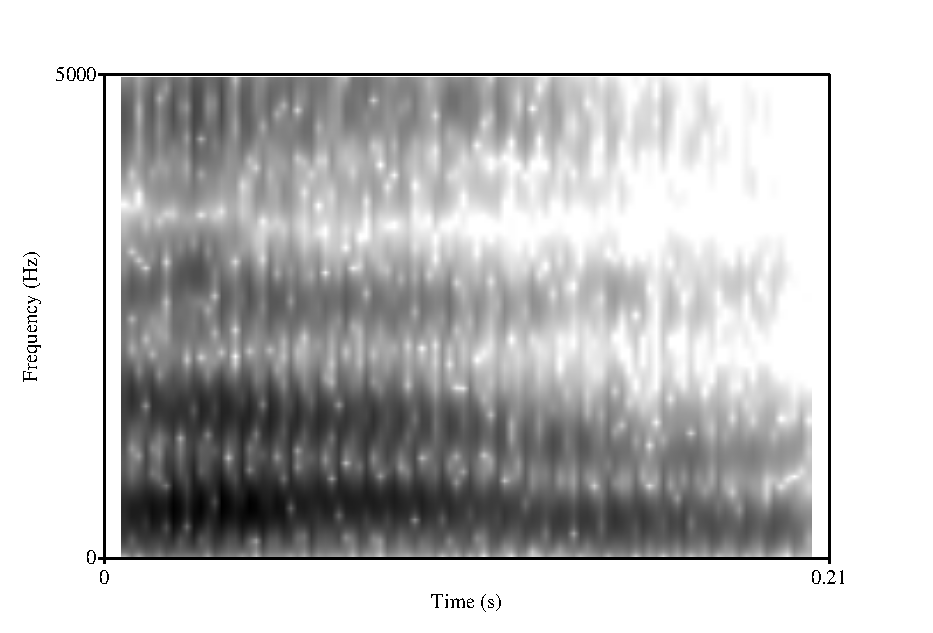
\includegraphics[scale=0.3,keepaspectratio]{goat.eps}
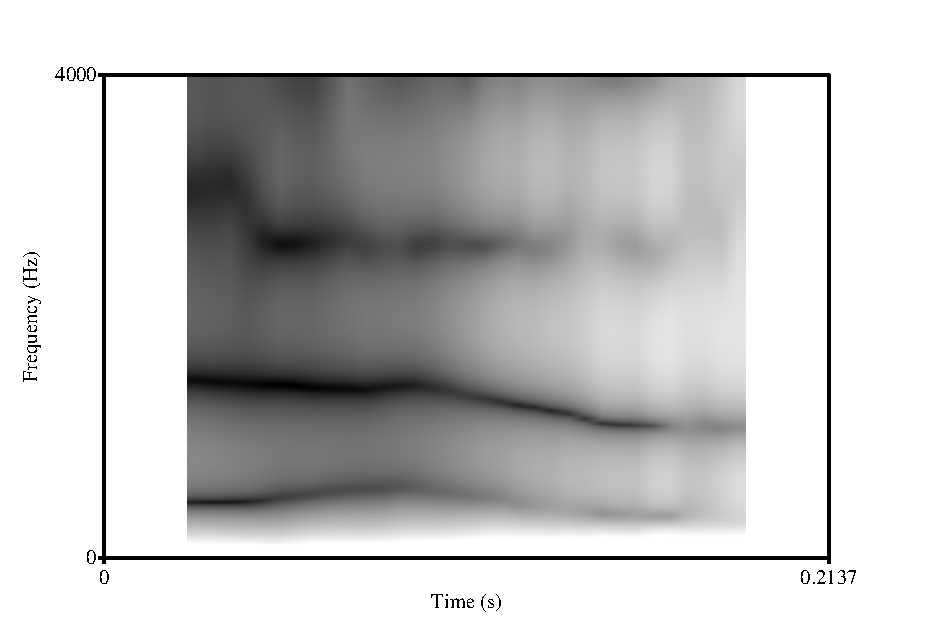
\includegraphics[scale=0.3,keepaspectratio]{LPC_filter.eps}
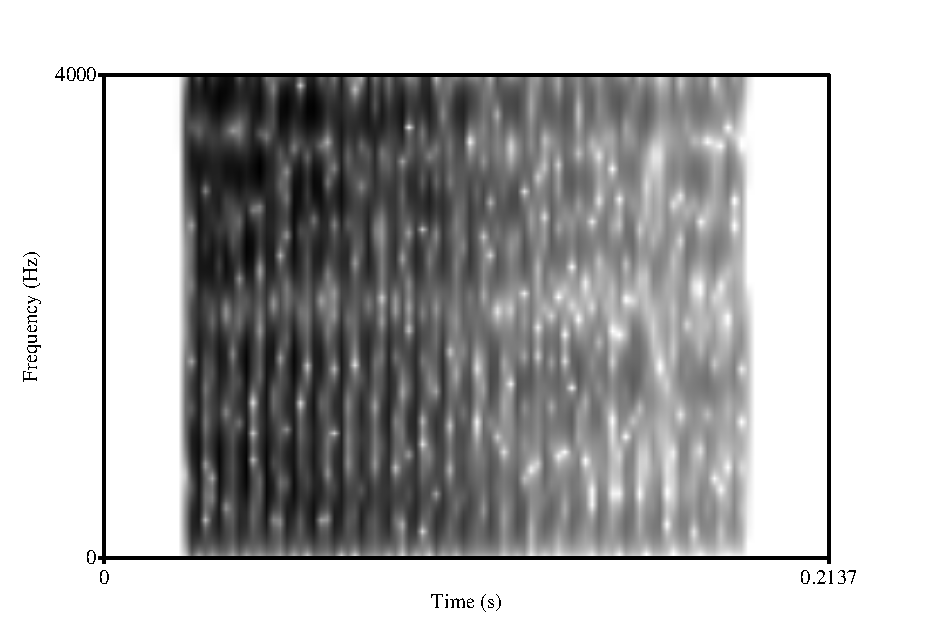
\includegraphics[scale=0.3,keepaspectratio]{source.eps}
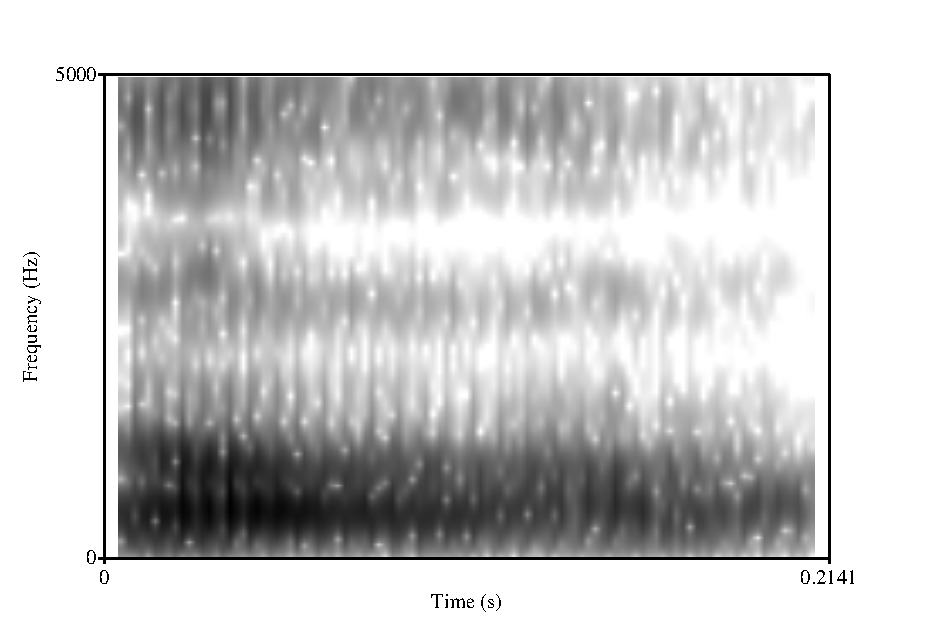
\includegraphics[scale=0.3,keepaspectratio]{goat_mono.eps}
\caption{Top right: Original vowel token; Top left: Smoothed spectrogram; Bottom left: Estimated glottal source; Bottom right: Resynthesized vowel}
\end{figure}
\newpage
In reality, there are a couple of difficulties with this method. Firstly, achieving full separation of the source and filter representations is very difficult. If this stage doesn't work properly, the stimuli may contain `phantom' formants, left over from the original speech token. To solve this problem, Alku (1996) has developed a method for highly accurate source estimation, which basically involves using the inverse filtering process iteratively. Figure three shows the difference -- you should see that Alku's (1996) method results in a much `whiter' spectrogram, with very little evidence of residual formant-like bands.

\begin{figure}[!ht]
\includegraphics[scale=0.4,keepaspectratio]{not_very_white.png}
\includegraphics[scale=0.4,keepaspectratio]{much_more_white.png}
\caption{Left: spectrogram of inverse-filtered glottal source; Right: spectrogram of glottal source estimated using Alku's (1996) method}
\end{figure}

A second problem is that LPC decomposition usually results in the loss of the higher frequency component of the original sound. While this doesn't affect our perception of vowel quality, it makes the stimuli sound quite muffled, and causes issues when we want to place the synthesized vowels in a consonantal context. To solve this problem, the high frequency component of the original sound can be added to the synthesis output (credit for this idea goes to Matt Winn -- mattwinn.com)

\begin{figure}[!ht]
\includegraphics[scale=0.4,keepaspectratio]{vowel_LF_only.png}
\includegraphics[scale=0.4,keepaspectratio]{vowel_HF_restored.png}
\caption{Left: spectrogram of resynthesized vowel showing frequencies up to 24KHz; Right: resynthesized vowel with higher frequencies restored.}
\end{figure}

Restoring the higher frequency component of the original signal improves the naturalness of the resulting stimuli considerably, and allows the resynthesized vowels to be placed in consonantal contexts without the need to downsample the carrier tokens.

\section*{Estimating Continuum Steps}

Now that we have established a method for generating the stimuli, all that remains is to decide how to calculate the formant values for the stimuli items. One thing we might want to do is create a continuum between two endpoints -- for example, we might want to create a continuum between \textipa{[i]} and \textipa{[u]} for an experiment investigating the perception of vowel fronting.

\begin{figure}[!ht]
\centering
\includegraphics[scale=0.3,keepaspectratio]{i.png}
\includegraphics[scale=0.3,keepaspectratio]{u.png}
\caption{Left: spectrogram of natural token of \textipa{[i]}; Right: spectrogram of natural token of \textipa{[u]}}
\end{figure}
The method for doing this is fairly intuitive. First, we match the two samples in the time domain by stretching or shrinking one of them using an algorithm called \textit{Time-Domain Pitch-Synchronous Overlap and Add}, which allows the length of a sound to be modified without pitch being affected.
\begin{figure}[!ht]
\centering
\includegraphics[scale=0.3,keepaspectratio]{original_i_token.png}
\includegraphics[scale=0.3,keepaspectratio]{original_u_token.png}
\caption{Duration-matched vowel tokens. Left: \textipa{[i]}; Right: \textipa{[u]}}
\end{figure}
The formants can now be estimated using LPC analysis -- since the signals are matched in the time domain, this should result in a similar number of estimated formant points. The target values for each point can be estimated by interpolating between the two tokens.
\begin{figure}[!ht]
\centering
\includegraphics[scale=0.4,keepaspectratio]{distances.png}
\includegraphics[scale=0.4,keepaspectratio]{F2_continuum.png}
\caption{Example of interpolation of the second formant -- distances are measured at a number of time points, allowing intermediate values to be calculated at equal steps}
\end{figure}

The spectrogram below shows an eight-step continuum from \textipa{[i]} to \textipa{[u]} generated in this manner:

\begin{figure}[!ht]
\centering
\includegraphics[scale=0.7,keepaspectratio]{continuum_spec.pdf}
\caption{Eight step semisynthetic vowel continuum}
\end{figure}


\newpage
\section*{Example scripts}
These scripts are included to encourage others to learn about the methods discussed here. Please feel free to use them in your teaching and research, and do get in touch if you have any questions or comments regarding them.
\subsection*{klatt\_ipa\_vowels.praat}
I have included this to demonstrate the output of typical (fully-synthetic) speech synthesis. This script generates a set of synthetic IPA vowels based on the formant values provided on Bruce Hayes' website (\url{http://www.linguistics.ucla.edu/people/hayes/103/Charts/VChart/}). To use the script, just run it in Praat -- a sound and textgrid containing the vowels should appear in the objects window.
\subsection*{iaif\_ipa\_vowels.praat}
This script does the same thing as the one above, but uses a voicing source estimated from natural speech. I have included it to demonstrate the considerable increase in naturalness that this method brings. To use the script:
\begin{enumerate}
\item{Record yourself saying a word with a clear vowel}
\item{Click `View \& Edit' to view your recording, and select the vowel portion.}
\item{Click `File', then `Extract selected sound (time from 0)'}
\item{Close the editor window}
\item{Select the extracted sound in the objects window}
\item{Run the script}
\end{enumerate}
You should find a sound and TextGrid object in the objects window, which contain the semisynthetic vowels.
\subsection*{formant\_manipulation\_iaif.praat}
This script creates semisynthetic vowel continuua and embeds them in natural consonantal contexts. To use it, you need two tokens of the desired work which represent the endpoints of the continuum. Record or open those in Praat, then run the script. The script should prompt you through the following steps:
\begin{enumerate}
\item{The script will prompt you to select the `A' token for your continuum. This is the one which will be used when estimating the glottal source. Select the sound in the objects window, and click `continue'}
\item{The script will ask you how it should create the `B' endpoint. You can either choose to modify the original, or choose to select an existing sound from the objects window.}
\item{If you have chosen to use a natural sample for the `B' endpoint, you will now be prompted to choose it in the objects window.}
\item{The script will display a `manipulation' window, with its estimation of the pitch contour of the target token. If you wish to modify the pitch pattern, you can do so by clicking on the green dots and moving them as you wish. Otherwise, click `Continue'}
\item{The script will prompt you to select the target segments in the `A' and `B' tokens. Segment the vowel carefully, and click `Continue'.}
\item{The script will ask you how you would like to generate the preceding and following context. You can choose to use silence, or choose to extract the context from token `A' or `B'.}
\item{If you have chosen to extract the context from the speech samples, you will see the editor window again and be asked to select the preceding and following contexts.}
\item{The script will display an Intensity editor -- changes can be made here if desired; click `Continue' when ready.}
\item{The script will ask you to check and modify FormantGrid objects for the `A' and `B' token targets. At this stage, you should check that no errors have been made in the formant estimation. The formant contours can be modified by clicking on and moving the blue dots; alternatively, you can select the FormantGrid in the objects window and choose `Modify...Formula (frequencies)' to make changes to whole formant.}
\item{The script will produce a set of IPA vowels. Listen to these to judge the quality of the source-filter separation; if you hear any pops or squeaks, try running the script again, and perhaps consider using another natural sample. If the vowels sound OK, click `Continue'}
\item{You should find a sound and TextGrid file containing your continuum in the objects window.}
\end{enumerate}
\end{document}